% !TeX spellcheck = en_US
\chapter{Implementation}\label{ch:implementation}

This chapter will explain how the different approaches of Ch.~\ref{ch:approach} have been implemented.

\section{GRP vs HDT}\label{sec:implementationGRPvsHDT}

In this section, it will be explained how the comparison between HDT and GRP is implemented.
\todo{alles neu machen}

As has just explained, HDT can compress a graph that is similar to a hub pattern (few subjects, many objects) very well. So it gets worse the further away the graph is from this pattern. This corresponds to the authority pattern, where there are few objects but many subjects.

The task now is to create a series of RDF graphs that first correspond to the hub pattern and then continue to change in the direction of the authority pattern. This is illustrated in Fig.~\ref{fig:star_pattern}. In this scenario all graphs ($G_1$ to $G_m$) have the same size, i.e. the same number of nodes and edges. $G_1$ has only one subject connected to all objects. $G_2$ then has two subjects more and correspondingly 2 objects less. This goes on and on until there is only one object that is connected to all subjects ($G_m$). The edges are randomly distributed among the nodes, so that all nodes have a similar degree and each node has at least a degree of one.

\begin{figure}[h]
	\centering
	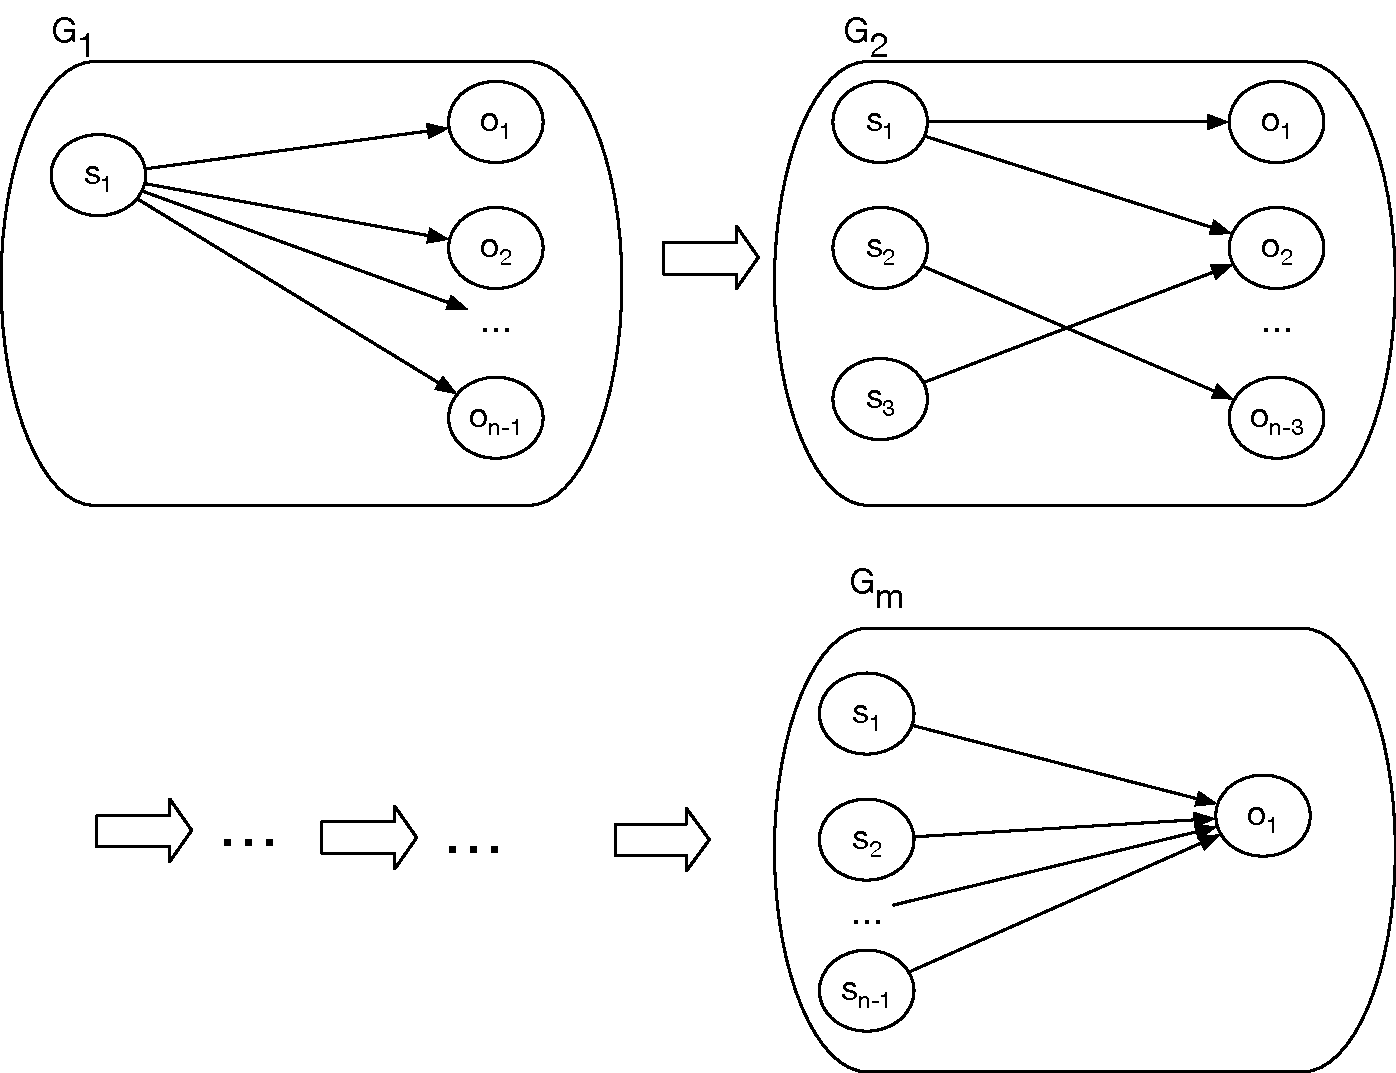
\includegraphics[width=0.8\textwidth]{figures/GRPvsHDT/starpattern.pdf}
	\caption{Step-by-step transition from hub pattern to authority pattern. The number of nodes $n$ is the same for each graph. The number of edges is also the same for each graph.}
	\label{fig:star_pattern}
\end{figure}

It is also ensured that each of the generated files has exactly the same size. This is made possible by ensuring that each URI has the same length. Since the RDF graph also has the same number of triples, the files are of the same size. Since the evaluation compares the compression ratios for the different RDF files, it is important that all files are of the same size to ensure a fair comparison.

A section of such a file (for $G1$) is shown in Fig.~\ref{fig:rdfFile}. In that example, there is only one distinct predicate for all triples. The number of predicates is always one at first. The amount of predicates has a similar effect on both compressors and is therefore omitted at first. But in Ch.~\ref{sec:evalHDT} that effect will be discussed in more detail.

Apart from that, blank nodes and literals are not used here. For both compressors, blank nodes and literals are being handled analogously to URI nodes. Therefore they are not needed at this point, in order to show the behavior of HDT and GRP in the above described scenario.

\begin{figure}[h]
	\centering
	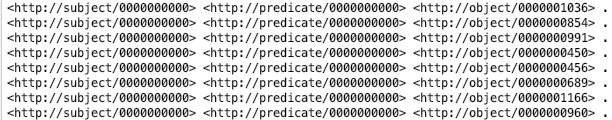
\includegraphics[width=0.8\textwidth]{figures/GRPvsHDT/file.png}
	\caption{Excerpt from the generated RDF file for $G_1$ (see Fig.~\ref{fig:star_pattern}). Each triple has the same length.}
	\label{fig:rdfFile}
\end{figure}

\section{Compression Improvements}\label{sec:implementationComprRatioImprovements}

This chapter introduces the implementation details of Ch.~\ref{sec:approachComprRatioImprovements}. First, applying ontology knowledge in order to achieve a better compression ratio is discussed. Afterwards, implementation details of the dictionary compression improvements are presented.

\subsection{Datasets}\label{sec:implementationDatasets}

Here, an overview about the different datasets, that have been used for the evaluation, is given. Although the datasets are used in Ch.~\ref{ch:evaluation}, they are presented here, since some implementation details are dependent on the data.

\subsubsection{Semantic Web Dog Food}

Semantic Web Dog Food~\footnote{http://www.scholarlydata.org/dumps/} is a collection of RDF files from the RDF researchers community. It contains data about their conferences and workshops.

\subsubsection{DBPedia}

DBPedia~\footnote{https://wiki.dbpedia.org/Downloads2015-04} is an RDF version of the knowledge from Wikipedia. It contains many different data files of a quite big size, with some of them having hundreds of millions of triples. Also, DBPedia includes an ontology that is used for the evaluation.

\subsubsection{Wordnet}

Wordnet contains knowledge about the English language. Words that have the same meaning are grouped in to the same \enquote{synset}. Those sets are the nodes in an RDF graph and relations between them are edges/properties.

\subsection{Ontology Knowledge}\label{sec:implementationOntKnowledge}

This chapter is about how to manipulate the RDF graphs to match the properties of Ch.~\ref{sec:approachOntKnowledge}. For this the query language SPARQL~\cite{sparql} is used.


\subsubsection{Overall Process}
Now, the overall process of applying ontology knowledge and evaluating whether it results in a better compression is explained. The several parts of the process will be discussed in the next sections. Fig.~\ref{fig:overallprocess} shows how it is implemented. First, the original graph or sub graph (the reason for sub graphs is explained below) is given to GRP. That part is called $in_1$ in Fig.~\ref{fig:overallprocess} and it will deliver the first result $out_1$.

In the next step, relevant properties have to be determined and the original graph will be manipulated. Then the manipulated graph is given to GRP. In addition, the relevant ontology triples have to be compressed and stored as well. Otherwise, the original graph could not be restored. Both graphs together are called $in_2$ which is then compressed by GRP and that delivers $out_2$.

Finally, $|out_1|$ and $|out_2|$ have to be compared. Here, the output sizes have to be compared instead of the compression ratios, because the ratio of $out_2$ would be relative to $in_2$. But a comparison to the original RDF graph ($in_1$) is needed in order to evaluate whether the manipulations delivered an improvement.

\begin{figure}
	\centering
	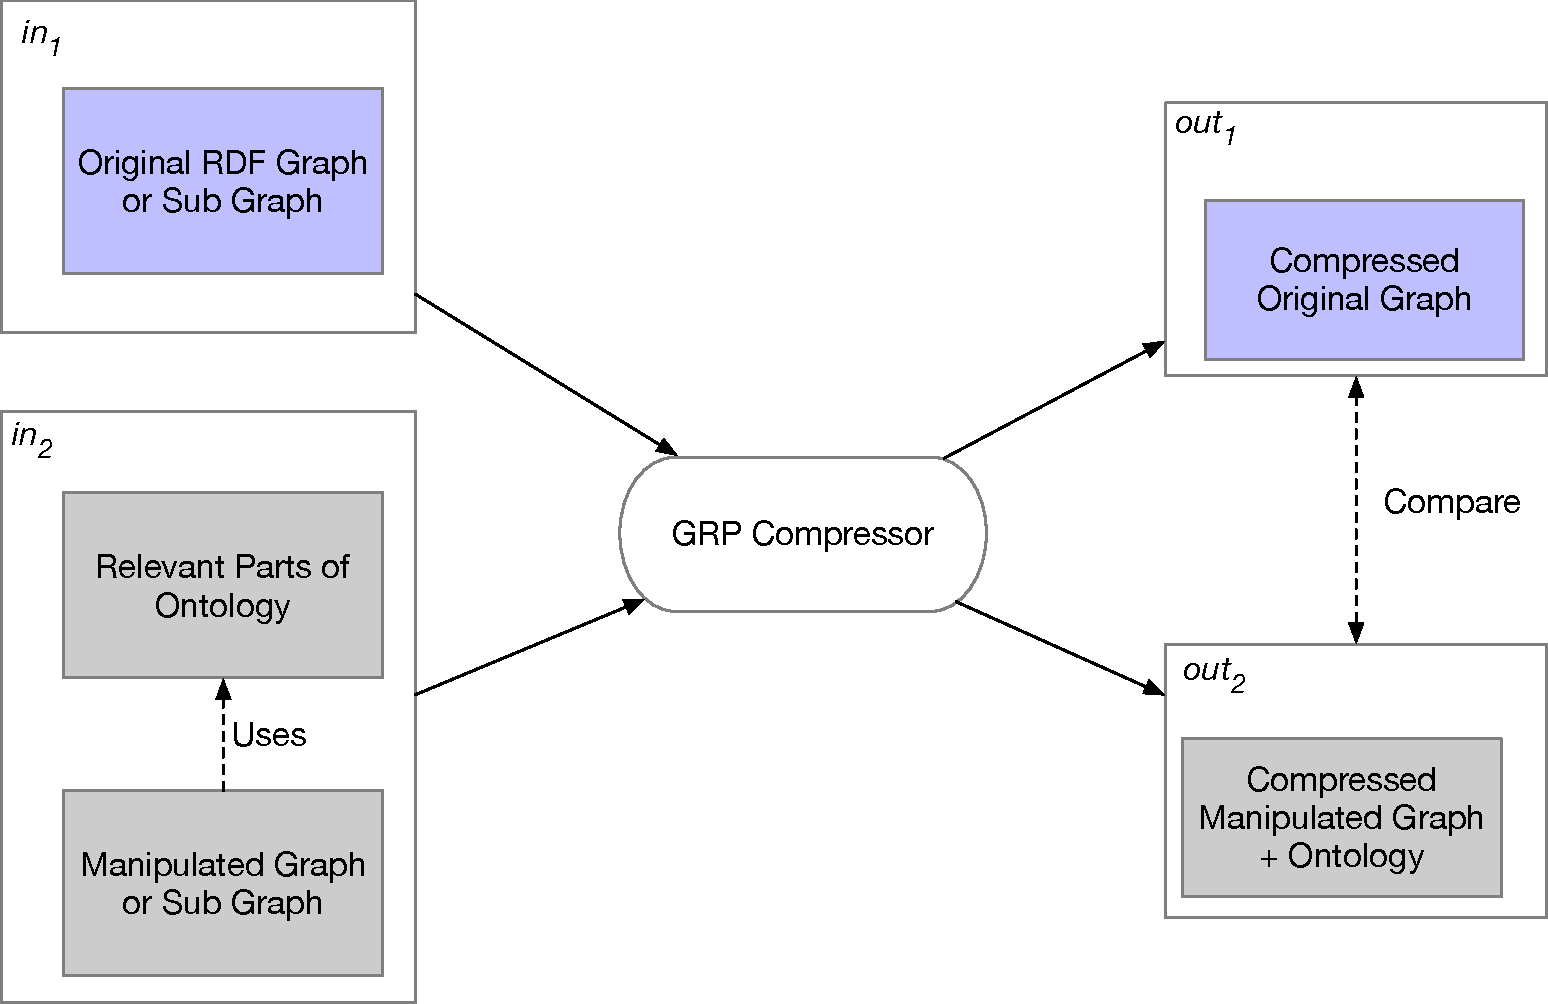
\includegraphics[width=0.9\linewidth]{figures/4_implementation/overallProcess}
	\caption{Overall process of applying ontology knowledge and comparing the compression results.}
	\label{fig:overallprocess}
\end{figure}

The process must be executed for the different manipulation aspects (symmetric, inverse etc.) independently. So there is one manipulated graph where all symmetric edges are added or removed, and analogously for the other manipulations. Finally, it is also possible to execute the process for one graph in which all different manipulations have been applied. 

In this way one sees first, what the manipulations bring individually and in the end also, what they all achieve in combination.


\subsubsection{Gathering Relevant Properties}
First, all relevant properties must be determined. This information should normally be directly contained in the ontology of the data, by triples of the form:

\[
\text{ {\tt <myProperty> <rdf:type> <owl:SymmetricProperty> .}}
\] 

This triple states that {\tt myProperty} is symmetric. The concept is analogous for inverse or transitive properties. 

However, this is not the case with DBPedia. In their ontology such triples do not occur for the symmetric or inverse cases (only for transitive properties). Symmetric and inverse properties have to be determined in a different way. In DBPedia's ontology the equivalent properties of Wikidata~\footnote{https://www.wikidata.org/wiki/Wikidata:Main\_Page} are given. Now one can check in the Wikidata ontology whether the properties are symmetric or inverse, because there the information is given.

In Wordnet, transitive properties are explicitly given, but symmetric and inverse are not. It is necessary to determine them by understanding the meaning of Wordnet's relations. Properties connect different \enquote{synsets}. One of those properties is antonymy, which is like an opposite-relation between words. Therefore, the property can be seen as symmetric.

\todo{inverse bei wordnet}

After all symmetric properties have been found (they are shown in Ch.~\ref{ch:evaluation}), manipulations to the graph have to be executed.

\subsubsection{Symmetric Properties}

In order to remove or add symmetric properties SPARQL can be used. The code of listing~\ref{lst:symmetricInsert} will be used to do add symmetric triples.

\begin{lstlisting}[captionpos=b, caption=SPARQL update for adding triples with the symmetric property p., label=lst:symmetricInsert,
basicstyle=\ttfamily,frame=single,float=hbt,]
INSERT {?o ?p ?s}
WHERE{
	{?s ?p ?o}
	MINUS {?o ?p ?s}
}
\end{lstlisting}

That update has to be executed for each symmetric property $p$. In the case where one wants to remove the second, a delete update would have to executed. That delete is shown in Listing~\ref{lst:symmetricDelete}.


\begin{lstlisting}[captionpos=b, caption=SPARQL update for removing triples with the symmetric property p., label=lst:symmetricDelete,
basicstyle=\ttfamily,frame=single,float=hbt,]
DELETE {?o ?p ?s}
WHERE{
?s ?p ?o .
FILTER (EXISTS {?o ?p ?s } && (str(?s) > str(?o) )
}
\end{lstlisting}

Here one has to be careful not to delete both directions, this can be done by using a filter.

\subsubsection{Inverse Properties}

Assume that $ p1 $ and $ p2 $ are inverse properties. Listing~\ref{lst:inverseInsert} is used to add the triple $(o,p1,s)$ if $(s,p2,o)$ already exists. That update has to be made in both directions  
\[
(p1,p2) \text{ and } (p2,p1)
\]
, in case the other direction exists. If one wants to remove triples instead of adding them, a delete has to be performed which is shown in Listing~\ref{lst:inverseDelete}

\begin{lstlisting}[captionpos=b, caption=SPARQL update for adding triples with the inverse properties p1 and p2., label=lst:inverseInsert,
basicstyle=\ttfamily,frame=single,float=hbt,]
INSERT {?o ?p1 ?s}
WHERE{
	{?s ?p2 ?o}
	MINUS {?o ?p1 ?s}
}
\end{lstlisting}



\begin{lstlisting}[captionpos=b, caption=SPARQL update for removing triples with the inverse properties p1 and p2., label=lst:inverseDelete,
basicstyle=\ttfamily,frame=single,float=hbt,]
DELETE {?o ?p1 ?s}
WHERE{
?s ?p2 ?o .
FILTER (EXISTS { ?o ?p ?s })
}
\end{lstlisting}

\subsubsection{Transitive Properties}

Here one wants to remove the triple $(s,p,o)$ if there exists a path from $s$ to $o$ via the transitive predicate $p$ of a length of at least two edges. That can be achieved by Listing~\ref{lst:transitiveRemove} in which a property path is used in the first line of the where clause.

Of course, it is also possible to add the triple $(s,p,o)$ if it does not exist. That can be done similarly with an insert and is shown in Listing~\ref{lst:transitiveInsert}.

\begin{lstlisting}[captionpos=b, caption=SPARQL update for removing triples with the transitive property p., label=lst:transitiveRemove,
basicstyle=\ttfamily,frame=single,float=hbt,]
DELETE { ?s ?p ?o }
WHERE { 
	?s ?p/?p+ ?o. 
	?s ?p ?o 
}
\end{lstlisting}


\begin{lstlisting}[captionpos=b, caption=SPARQL update for adding triples with the transitive property p., label=lst:transitiveInsert,
basicstyle=\ttfamily,frame=single,float=hbt,]
INSERT { ?s ?p ?o }
WHERE { 
?s ?p/?p+ ?o. 
FILTER (NOT EXISTS {?s ?p ?o })
}
\end{lstlisting}

\subsubsection{Sub Graphs}

Real datasets are quite big and it can happen that there are only a few relevant properties (symmetric/inverse/transitive). Even if there are many of those properties it can be that they do not occur often in the data. In that case, the effect of manipulating the data can not have a big impact on the compression ratio. However, one still wants to investigate if the effect is possibly there. Therefore, it is necessary to form a smaller graph in which those relevant properties occur often. So, a procedure to build a sub graph is needed.

First, all triples $t_1,...,t_n$ are collected which contain one of the relevant properties. It would now be possible to randomly add a number of remaining triples in order to get a more diversified graph. But that would result in a graph far away from the original and would probably not contain structural patterns from the original one.

Therefore, we choose to add triples that are directly connect to the subjects or objects of $t_1,...,t_n$. By doing that, a real sub graph is extracted out of the original graph.

The procedure is illustrated in Fig.~\ref{fig:subgraph}. There $p$ is the only relevant property. Consequently, the green triples are collected in the first step. The red triples are collected in the second step, because they are connected to triples from the first step.

\begin{figure}
	\centering
	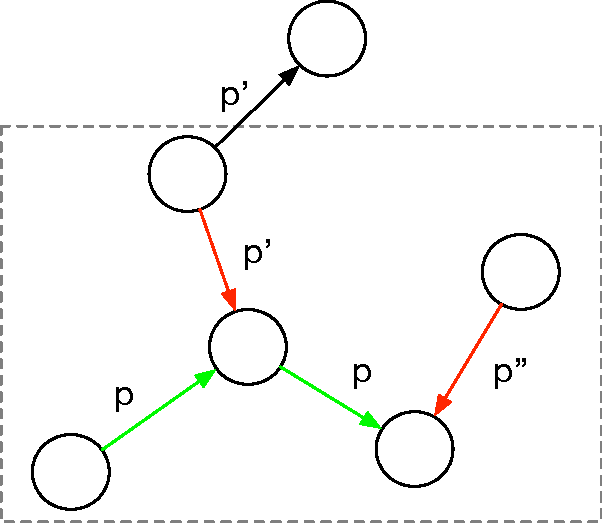
\includegraphics[width=0.4\linewidth]{figures/4_implementation/subgraph}
	\caption{Extraction of a sub graph (marked by dashed line).}
	\label{fig:subgraph}
\end{figure}



\subsection{Dictionary Improvements}\label{sec:implementationDictImprovements}

For the dictionary improvements, HDT's dictionary compression is used as a basis. Therefore, the HDT-Java code~\footnote{https://github.com/rdfhdt/hdt-java} has been extended.

\subsubsection{Literals}\label{sec:implementationLiterals}

As already mentioned in Ch.~\ref{sec:approachDictImprovements}, the literals will be compressed using a Huffman code. To achieve that, HDT is changed such that it does not compress literals by prefix trees, but rather gives the literals to the newly created {\tt HuffmanHandler}, which compresses all literals and finally stores them in a binary format. In order to make that possible, the {\tt HuffmanHandler} has to traverse all literals in the beginning of the compression to establish a Huffman Tree.

In addition, the Huffman code/tree itself has to be stored in order to be able to decompress the data. There is no standard way for storing the binary tree. One approach can be seen in Algorithm~\ref{alg:HuffmanEncode} which has to be started with the root node. That method creates an unambiguous bit representation of the tree. It traverses the tree in a depth-first-search-manner and writes a one and the current node's character in case the current node is leaf. Otherwise it writes a zero and the procedure is then called recursively for the current node's children. This encoding is unambiguous, because each node is either a leaf or has exactly two children.

\begin{algorithm}
	\caption{EncodeNode (TreeNode node)}\label{alg:HuffmanEncode}
	\begin{algorithmic}[1]
		\If{node is leaf}
		\State writeBit(1)
		\State writeCharacter(node.character)
		\Else
		\State writeBit(0)
		\State EncodeNode(node.leftChild)
		\State EncodeNode(node.rightChild)
		\EndIf
	\end{algorithmic}
\end{algorithm}


Alternatively, there are pre-computed Huffman trees for natural languages such as English. There, it has already been investigated which letter occurs how often in English texts and in this way a generally valid Huffman code has been established. The advantage is that one does not have to save the Huffman tree and does not have to calculate it oneself, which saves runtime. The disadvantage, however, is that the tree is not optimal for the text to be compressed, as it is more general. Another problem in our case is that the literals contain a lot of special characters that are not taken into account in prefabricated Huffman codes. Therefore, prefabricated codes will not be used.

\subsubsection{Blank Nodes}\label{sec:implementationBlankNodes}

HDT normally uses the arbitrary and long strings generated by the Jena API and tries to compress them using prefix trees.

Now, two approaches, which have both been implemented, for improving the compression of blank nodes are presented.

The first approach is to use shorter IDs (e.g. numbers from 1 to $n$). Then, during the run time a mapping from old ID to new ID is maintained in order to make sure that the same blank node will get the same new ID if it occurs multiple times. That mapping does not have to be stored persistently and will therefore be omitted once the compression is finished.

The second approach is to omit blank node IDs completely. The HDT code is changed in such a way that skips blank nodes in the process of storing the dictionary.

















